\chapter{Conclusions and Future Work} \label{chapter:conclusion}

Enabled by energy harvesting and low-power computing techniques, IPSs are expected to be a promising system paradigm for numerous IoT sensors in the near future, with forecasts of hundreds of billions being installed~\cite{sparks2017trillion}.
IPSs adapt to the intrinsically variable and uncontrollable power input of energy harvesters, and thus, circumvent large volume, environmental impact, and limited lifespan of large energy buffers, i.e. batteries and supercapacitors, that contradict with the requirements of future IoT sensors.

While existing IPS technology has mainly focussed on the computing part, i.e. efficiently and correctly retaining the system state across power interruptions, this thesis has explored energy budgeting in IPSs. 
The energy budget in an IPS is represented as the energy allocated for an active cycle when the load wakes up and executes program. 
As the energy budget is determined by the energy storage size and the voltage threshold that wakes up the load, this thesis has conducted the research following the two aspects, where \cref{chapter:sizingeffect} and \cref{chapter:sizingapproach} explored the energy storage sizing effect and \cref{chapter:opta} proposed runtime profiling and adaptation of voltage thresholds. 

\correct{
\section{Answers to Research Questions}
}
% Recap of main work and findings in this thesis

\begin{enumerate}

\correct{
\item \textbf{What is the effect of sizing the energy storage capacity on IPS performance?}
}

To minimise device dimensions and interruption periods, most IPSs have adopted only a minimum amount of energy storage. 
However, as found in \cref{chapter:sizingeffect}, this can be energy inefficient as the system has to frequently save and restore the state. 
Hence, a reactive IPS model was proposed to explore the sizing effect of energy storage on forward progress. 
Derived from the pattern of operating cycles in IPSs, the proposed model can fast and accurately estimates forward progress given supply current and energy storage capacitance, facilitating exploration and understanding of IPSs. 
The proposed model was configured with experimentally profiled parameters on a reactive IPS platform.
The model was experimentally validated with a 0.5\% mean error across multiple conditions of supply current and energy storage capacitance. 
The energy storage sizing effect was then explored with respect to supply current and volatile state size, showing a forward progress improvement of up to 65\% compared to using minimised energy storage.
The forward progress improvement from sizing energy storage becomes significant when supply current is low and when volatile state size is large. 
Additionally, the energy storage capacitance that achieves the maximum forward progress improvement (i.e. \nm{C}{$\alpha$\_max} as denoted in \cref{chapter:sizingeffect}) can be 3.2$\times$ as large as the one that gains a 95\% improvement. 
With considerations on volume and charging time of a large capacitor, this indicates that an energy storage sizing approach is in need to comprehend multiple design factors in IPSs instead of maximising forward progress only.

\correct{
\item \textbf{How may the energy storage of IPSs be sized to trade off multiple design factors, such as forward progress, device dimensions, interruption periods?}
}

As indicated in \cref{chapter:sizingeffect}, an energy storage sizing approach for recommending an energy storage size considering multiple design factors when deploying IPSs was proposed in \cref{chapter:sizingapproach}.
Following a modelling and simulation process, the sizing approach is able to output forward progress, capacitor volume, and interruption periods given long-term energy source data, energy harvester configurations, and energy storage capacitance.
Through iterations with different capacitance values, the sizing approach trades off various properties of the system with a cost function and recommends an appropriate energy storage size. 
The sizing approach was configured and demonstrated with parameters profiled on an IPS and real-world data of indoor and outdoor PV sources. 
The results showed up to a 43\% annual forward progress gain by sizing energy storage.
Corresponding to \cref{chapter:sizingeffect}, this improvement is more significant with weaker power input, e.g. a smaller PV panel size. 
With an example cost function, the results showed that the suggested energy storage capacitance achieves 93\% of the maximum forward progress while saving 83\% capacitor volume and 91\% interruption periods, compared to the one that solely maximises forward progress.
Combining the findings in \cref{chapter:sizingeffect} and \cref{chapter:sizingapproach}, the conclusion is that energy storage should be carefully designed, rather than minimised or indiscriminately picked, to efficiently operate IPSs. 

\correct{
\item \textbf{How can an IPS run safely and efficiently when executing tasks with runtime-variable energy consumption?}
}

While the energy storage size studied, \cref{chapter:opta} has focussed on the voltage thresholds of an energy budget. 
With the runtime variability of energy consumption, the prior SoA approaches can cause non-termination or reduce system energy efficiency.
The variable energy consumption has been exemplified in four cases, which are variable data sizes, variable peripheral configurations, device variability, and capacitor ageing. 
Motivated by this variability, \nn{}, a runtime energy profiling and adaptation method, was presented in \cref{chapter:opta}. 
\nn{}'s runtime energy profiling measures $\Delta\nmm{V}{task}$, the drop of supply voltage caused by a task without any incoming energy meanwhile, with supply connected to save the input energy during profiling.
To obtain $\Delta\nmm{V}{task}$, it measures the input current before the task and compensates the supply voltage difference of executing a task by the input current.
Utilising the runtime energy profiling method, \nn{}'s runtime energy adaptation adapts the voltage threshold for a task, efficiently allocating a barely sufficient threshold according to its runtime energy consumption. 
\nn{}'s runtime energy adaptation also provides an option of linearly scaling the threshold by user-defined parameters, allowing a fast switching of thresholds without excessive profiling. 
\nn{} was implemented on a TI MSP430FR5994 MCU with an external supply voltage monitor. 
The experimental results has shown multiple findings as follows.
\nn{}'s runtime energy profiling has a low error within \SI{5}{\milli\volt}, enabling IPSs to perform energy profiling at runtime and alleviating manual profiling efforts.
\nn{} can adapt its threshold for a new task or on a new device. 
\nn{} is also able to cope with an increased $\Delta\nmm{V}{task}$ from increased energy consumption or capacitor ageing, where it survived with up to 68\% capacitance reduction while the SoA failed, allowing IPSs to operate beyond capacitor lifetime. 
Finally, \nn{} efficiently adjusts to a barely sufficient threshold with variable data sizes, which lowers operating voltage and improves energy efficiency, thus improving up to 98\% progress over the SoA approaches.

\end{enumerate}

% \section{Answers to Research Questions}
% \todo[inline]{Answers to research questions?}

\section{Future Work}

While this thesis has presented extensive research work contributed to the energy budgeting in IPSs, some interesting research topics can be explored in the future so as to achieve a more energy-efficient IPS. 
One interesting research research could be: \textit{can IPSs transform from an MCU-centred system to an EMU-centred system, i.e. powering the load modules in a controllable and programmable order?} 

Currently, an off-the-shelf energy management unit (EMU) for energy harvesting applications, e.g. TI BQ25504~\cite{bq25504}, has the major features of boost charging, voltage detection, and power gating.
Due to its features, an EMU can improve the energy efficiency of an IPS typically with low power input, where energy can be collected from a very weak supply (e.g. \SI{130}{\milli\volt} input voltage) at a low quiescent current draw (e.g. \SI{330}{\nano\ampere}). 
While energy management makes a significant impact on IPS performance as illustrated in this thesis, published IPS approaches are implemented on an MCU, where the MCU may interface with an EMU.
To cope with the intermittent power supply, the MCU manages computing state and stored energy while executing application software, which deviates from what a processor is initially designed for. 

It could be worthwhile to explore a dedicated EMU for IPSs that manages energy and state with power-gating on load modules.
% Benefits. 
A major benefit of this could be a lower quiescent current consumption. % Why not a MCU with additional power gates?
External peripherals in existing MCU-centred IPSs are powered together with the MCU as a unified load.
This increases the quiescent or sleep current when the system waits for energy to refill, especially with more peripherals connected or peripherals with large quiescent current consumption. 
With an EMU-centred IPS, each load module is power-gated and only powered when it is due to work. 
Thus, the system can work with a lower input current, ensuring the operation of IPSs in a poor energy condition. 
Other advantages could include (i) a lower control overhead as the IPS software could be offloaded to hardware, (ii) each module can independently work without a processor being active immediately before and after the operation of a module, and (iii) an integral IPS hardware that saves the area overhead of external components. 

\begin{figure}
    \centering
    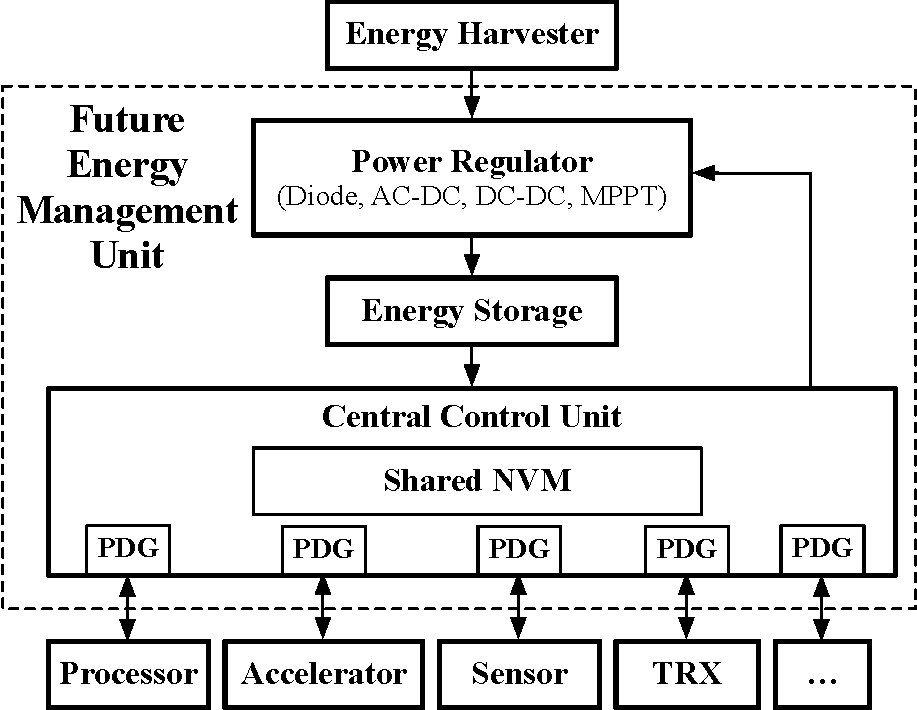
\includegraphics[width=0.9\columnwidth]{ch6_conclusion/figures/EMUIPSarch.pdf}
    \caption{A conceptual architecture of an EMU-centred IPS.}
    \label{fig:emuips}
\end{figure}

A conceptual architecture of such an EMU-centred IPS is depicted in \fref{fig:emuips}.
The central control unit is responsible for the configuration of input power regulation (e.g. MPPT), control of which module to power, and the data flow among modules through a shared NVM. 
\correct{The load modules, such as accelerators, sensors, and wireless transceivers (TRX), are connected to the EMU through a power gate (PG). }
The central control unit opens a corresponding PG when a load module is supposed to work.
The load modules communicate through the shared NVM, where the volatile state and shared data are saved. 
The concept could be possibly achieved by incorporating IPS functions (e.g. state consistency) into existing EMUs.
This may reconstruct the hardware architecture of existing IPSs.

Some potential subdivided research questions related to this topic could be:
\begin{enumerate}
    \item Is an EMU-centred IPS theoretically more energy-efficient than existing MCU-centred IPSs considering the energy trade-off, e.g. initialisation overheads of modules vs. energy savings of power-gating?
    \item How could an EMU-centred IPS be implemented?
    \item Is it possible to integrate the functions of IPSs into a dedicated IC?
    \item How can such a system be programmed so that it can have a configurable control logic?
    \item Is a new programming model necessary for an EMU-centred IPS?
    \item How can the system state be retained across multiple modules in a shared NVM?
    \item Could an EMU-centred IPS condition the supply voltage for each module such that modules with different operating voltage levels can cooperate? 
\end{enumerate}

\correct{
\section{Conclusion}

This thesis has presented extensive research work towards the energy budgeting for efficient operation of IPSs.
A reactive IPS model was proposed to reveal the sizing effect of energy storage on forward progress, emphasizing that adding a small amount of energy storage beyond the minimum can improve IPS performance.
A simulation tool was provided to estimate forward progress of IPSs given real environmental energy conditions, allowing an appropriate energy storage to be picked considering multiple design factors. 
To safely and efficiently execute atomic tasks, a method of runtime energy profiling and adaptation was presented, enabling IPSs to adapt wake-up voltage thresholds to variable energy consumption and future device degradation.
All software related to the research work in this thesis was open-source available, facilitating reproduction of results and future research.
To summarise, this thesis has contributed methods of energy budgeting to improve IPS performance alongside the existing research work on efficient state-retention techniques.
}